\documentclass[letterpaper,addpoints,answers]{exam}
\usepackage{graphicx}
\usepackage{multicol}
\usepackage{tikz}
\usetikzlibrary{scopes}

\makeatletter
\def\grd@save@target#1{%
  \def\grd@target{#1}}
\def\grd@save@start#1{%
  \def\grd@start{#1}}
\tikzset{
  grid with coordinates/.style={
    to path={%
      \pgfextra{%
        \edef\grd@@target{(\tikztotarget)}%
        \tikz@scan@one@point\grd@save@target\grd@@target\relax
        \edef\grd@@start{(\tikztostart)}%
        \tikz@scan@one@point\grd@save@start\grd@@start\relax
        \draw[minor help lines] (\tikztostart) grid (\tikztotarget);
        \draw[major help lines] (\tikztostart) grid (\tikztotarget);
        \grd@start
        \pgfmathsetmacro{\grd@xa}{\the\pgf@x/1cm}
        \pgfmathsetmacro{\grd@ya}{\the\pgf@y/1cm}
        \grd@target
        \pgfmathsetmacro{\grd@xb}{\the\pgf@x/1cm}
        \pgfmathsetmacro{\grd@yb}{\the\pgf@y/1cm}
        \pgfmathsetmacro{\grd@xc}{\grd@xa + \pgfkeysvalueof{/tikz/grid with coordinates/major step x}}
        \pgfmathsetmacro{\grd@yc}{\grd@ya + \pgfkeysvalueof{/tikz/grid with coordinates/major step y}}
        \foreach \x in {\grd@xa,\grd@xc,...,\grd@xb}
        \node[anchor=north] at (\x,\grd@ya) {\pgfmathprintnumber{\x}};
        \foreach \y in {\grd@ya,\grd@yc,...,\grd@yb}
        \node[anchor=east] at (\grd@xa,\y) {\pgfmathprintnumber{\y}};
      }
    }
  },
  minor help lines/.style={
    help lines,
    gray,
    line cap =round,
    xstep=\pgfkeysvalueof{/tikz/grid with coordinates/minor step x},
    ystep=\pgfkeysvalueof{/tikz/grid with coordinates/minor step y}
  },
  major help lines/.style={
    help lines,
    line cap =round,
    line width=\pgfkeysvalueof{/tikz/grid with coordinates/major line width},
    xstep=\pgfkeysvalueof{/tikz/grid with coordinates/major step x},
    ystep=\pgfkeysvalueof{/tikz/grid with coordinates/major step y}
  },
  grid with coordinates/.cd,
  minor step x/.initial=.5,
  minor step y/.initial=.2,
  major step x/.initial=1,
  major step y/.initial=1,
  major line width/.initial=1pt,
}
\makeatother


\begin{document}

\begin{coverpages}
 \large\bfseries
 
 \noindent 
 Physics 107: Physics for Life-Sciences

 \vspace{2ex}
 \noindent
 Midterm Exam: November 17, 2014

 \vspace{3ex}
 \noindent 
 This test is administered under the rules and regulations of the honor code of the College of William \& Mary.

 \vspace{2ex}
 \noindent 
 Name:\enspace\makebox[2.3in]{\hrulefill} \\

 \noindent 
 Signature:\enspace\makebox[2in]{\hrulefill} \\

 \vspace{5ex}
 \noindent 
 Instructions:
 \begin{itemize}
  \item This is a closed book, closed notes test.
  \item Calculators are permitted, but not laptops or cell phones. Devices with wireless connections are not allowed.
  \item Start your work from the fundamental equations on the formula sheet, and derive any additional expressions that you may need.
  \item Circle your answer for each part of each problem. 
  \item Clearly mark out any work that you wish the grader to disregard.  Do not waste your time erasing.
  \item Your work will be graded based on your ability to write down a logical and organized solution grounded in the correct assessment of the physics of a situation. No credit will be given for an answer that is not justified by a logical solution or where that justification is not organized or readable. Partial credit will be given up to the point where your solution departs from a correct analysis of the physics involved for any given part of a problem.
 \end{itemize}

 \pagebreak

 \begin{center}
  \gradetable[v][questions]
 \end{center}
 
\end{coverpages}
 

\begin{questions}

\question
A deli owner creates a lunch special display board by taking a uniform board which has a mass of 8.00~kg and positioning it with the dimensions as given in the figure (the chain is massless). The sign is standing in equilibrium on the sidewalk. Assume that there is no friction between the legs and the sidewalk.
\begin{center}
 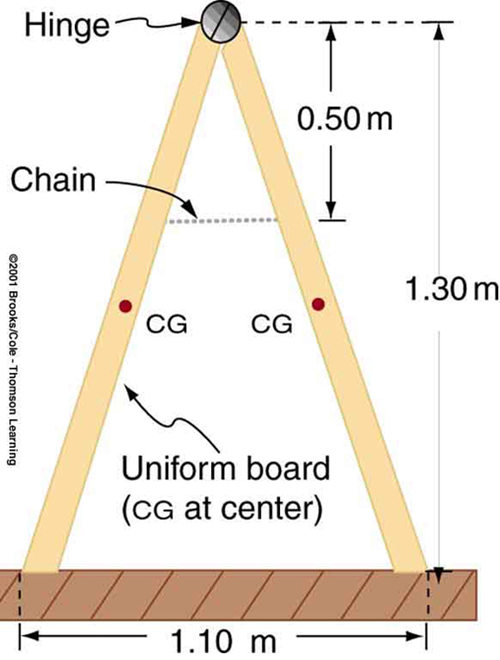
\includegraphics[width=0.28\textwidth]{test3/sandwich_board}
\end{center}
\begin{parts}
 \part[10] What is the tension in the chain?
 \vspace{22\baselineskip} 
 \part[10] What is the force exerted on each side of the hinge?
 \vspace{16\baselineskip} 
\end{parts}

\pagebreak

\question
\def\iangle{30} % Angle of the inclined plane
\def\arcr{0.75cm} % Radius of the arc used to indicate angles

Three objects are released from rest at the top of a ramp: a solid ball, a solid cylinder and a hollow cylinder.  They are all made out of aluminum with a density of $2700~\hbox{kg}/\hbox{m}^3$ and have the same radius of 10~cm.  Both cylinders have a length of 50~cm, and the hollow cylinder has a wall thickness of 2~mm (which you can ignore where appropriate).  The 1.00~m long ramp is at an angle of $\iangle^\circ$ with the horizontal.
\begin{center}
 \begin{tikzpicture}[
    force/.style={>=latex,draw=blue,fill=blue},
    axis/.style={densely dashed,gray,font=\small},
    M/.style={rectangle,draw,fill=lightgray,minimum size=0.5cm,thin},
    m/.style={rectangle,draw=black,fill=lightgray,minimum size=0.3cm,thin},
    plane/.style={draw=black,fill=blue!10},
    string/.style={draw=red, thick},
    pulley/.style={thick},
]
    %% Sketch
    \draw[plane] (0,-1) coordinate (base)
                     -- coordinate[pos=0.5] (mid) ++(\iangle:3) coordinate (top)
                     |- (base) -- cycle;
    \path (mid) node[rotate=\iangle,yshift=0.25cm] (M) {$L = 1.00$~m};
    \draw[pulley] (top) -- ++(\iangle+90:0.25) circle (0.25cm)
                   ++ (90-\iangle:0.5) coordinate (pulley);
    \draw[->] (base)++(\arcr,0) arc (0:\iangle:\arcr);
    \path (base)++(\iangle*0.5:\arcr+5pt) node[right] {$\alpha = \iangle^\circ$};
 \end{tikzpicture}
\end{center}


The moment of inertia of a solid sphere around its center is $I_{solid\,sphere} = \frac{2}{5} M R^2$, of a solid cylinder $I_{solid\,cylinder} = \frac{1}{2} M R^2$, and of a hollow cylinder $I_{hollow\,cylinder} = \frac{1}{2} M (R_{inner}^2 + R_{outer}^2)$, 
\begin{parts}
 \part[5] Which of the three objects will have the highest velocity at the bottom of the ramp?  Justify your answer without resorting to calculations.
 \vspace{8\baselineskip}
 \part[15] Using conservation of energy, calculate the velocity at the bottom of the ramp for each of the objects.
 \vspace{26\baselineskip}
\end{parts}


\pagebreak

\question
A fire hose has a diameter of 6.40~cm.  Suppose the hose carries a flow of $40.0~\hbox{l}/\hbox{s}$ (1~liter is a volume of 1~$\hbox{dm}^3$).  The hose goes 10.0~m up a ladder to a nozzle with an inside diameter of 3.00~cm.  The water has a density of $1.00~\hbox{kg}/\hbox{dm}^3$ and a viscosity of $1.00~\hbox{mPa}\cdot\hbox{s}$.
\begin{center}
 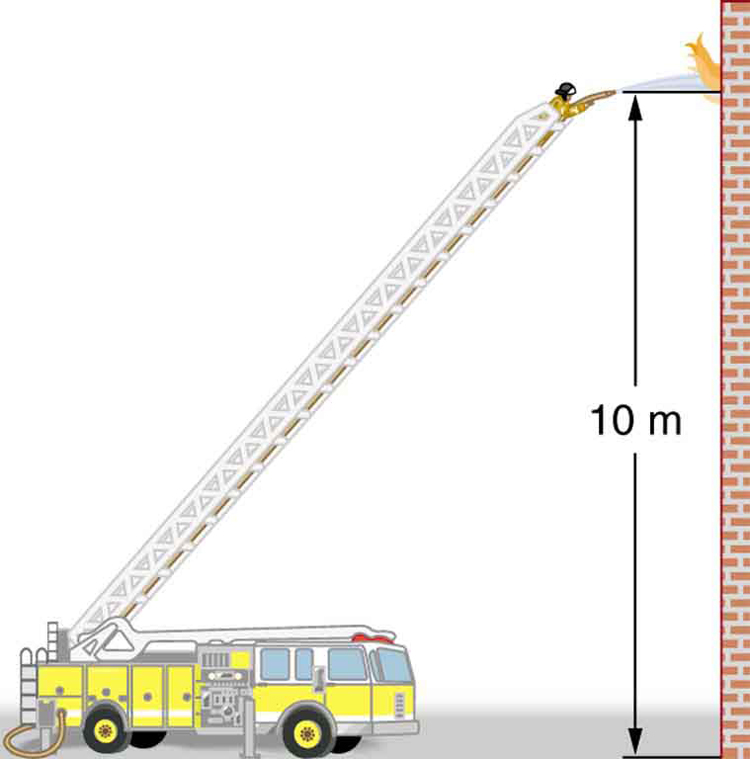
\includegraphics[width=0.3\textwidth]{test3/firehose}
\end{center}
\begin{parts}
 \part[5] What is the velocity with which the water will flow out of the nozzle?
 \vspace{12\baselineskip}
 \part[5] Will the flow in the fire hose be turbulent?
 \vspace{10\baselineskip}
 \part[5] Will the flow in the nozzle be turbulent?
 \vspace{10\baselineskip}
 \part[5] What must the gauge pressure in the fire engine be to sustain this flow?
 \vspace{18\baselineskip}
\end{parts}

\question[10]
Atmospheric pressure is sometimes expressed as 760~mm~Hg.  This means that atmospheric pressure can cause a column of mercury (Hg) to raise over 760~mm in a glass vacuum tube (pressure at the mercury surface is zero).  How high can atmospheric pressure cause a column of water to rise in a similar vacuum tube?  The density of mercury is 13.6~$\hbox{kg}/\hbox{dm}^3$ and the density of water is 1.00~$\hbox{kg}/\hbox{dm}^3$.
\vspace{12\baselineskip}

\end{questions}

 \pagebreak
 
 {\Large Possibly useful relations (feel free to detach this page):}
  
 \fontseries{\seriesdefault}
 \begin{multicols}{2}
 \large
 \noindent
 $\vec{v}_{avg} = \Delta\vec{x} / \Delta t$ \\
 $\vec{a}_{avg} = \Delta\vec{v} / \Delta t$ \\
 $v = v_0 + a t$ \\
 $v_{avg} = \frac{v_0 + v}{2}$ \\
 $x = x_0 + v_0 t + \frac{1}{2} a t^2$ \\
 $v^2 = v_0^2 + 2 a (x - x_0)$ \\
 $R = \frac{v_0^2}{g}\sin 2\theta$ \\
 $h = \frac{v_0^2}{2 g} \sin^2 \theta$ \\
 $\vec{F}_{net} = m \vec{a}$ \\
 $\vec{F}_{BA} = - \vec{F}_{AB}$ \\
 $\vec{W} = m \vec{g}$ \\
 $\vec{g} = 9.80\,$m/s$^2$ downward \\
 $0 \le f_s \le \mu_s N$ \\
 $f_k = \mu_k N$ \\
 $\frac{F}{A} = Y \frac{\Delta L}{L}$ \\
 $F_k = -k x$ \\
 $KE = \frac{1}{2} m v^2$ \\
 $W = F d \cos\theta$ \\
 $W_{\hbox{net}} = -\Delta PE$ \\
 $W_{\hbox{net}} = \Delta KE$ \\
 $PE_k = \frac{1}{2} k x^2$ \\
 $PE_g = m g h$ \\
 $KE_i + PE_i + W_{nc} = KE_f + PE_f$ \\
 $P = \frac{W}{\Delta t}$ \\
 $\hbox{Eff} = \frac{W_{out}}{E_{in}}$ \\
 $F_G = G \frac{m M}{r^2}$ \\
 $G = 6.67 \times 10^{-11}\,$N $\cdot$ m$^2$ / kg$^2$ \\
 $\vec{I} = \vec{F}_{avg} \Delta t$ \\
 $\vec{p} = m \vec{v}$ \\
 $\vec{F}_{net} = \frac{\Delta \vec{p}}{\Delta t}$ \\
 $v_1 - v_2 = v'_2 - v'_1$ \\
 $\theta = \frac{s}{r}$ \\
 $v = r \omega$ \\
 $f = \frac{1}{T}$ \\
 $\omega = 2 \pi f$ \\
 $a_c = \frac{v^2}{r} = r \omega^2$ \\
 $F_c = m\frac{v^2}{r} = m r \omega^2$ \\
 $KE_{rot} = \frac{1}{2} I \omega^2$ \\
 $I_{point} = M R^2$ \\
 $I_{disk} = \frac{1}{2} M R^2$ \\
 $I_{sphere} = \frac{2}{5} M R^2$ \\
 $\tau = r F \sin\theta = r_\perp F$ \\
 $\omega = \frac{\Delta \theta}{\Delta t}$ \\
 $\alpha = \frac{\Delta \omega}{\Delta t}$ \\
 $\tau = I \alpha$ \\
 $L = I \omega$ \\
 $\tau = \frac{\Delta L}{\Delta t}$ \\
 $P = \frac{F}{A}$ \\
 $P_{gauge} = P - P_{atm}$ \\
 $\rho = \frac{M}{V}$ \\
 $Q = \frac{\Delta V}{\Delta t} = A v$ \\
 $Q = \frac{\Delta P \pi r^4}{8 \eta L}$ \\
 $\hbox{Power} = P Q$ \\
 $A \cdot v = \hbox{constant}$ \\
 $P + \rho g y + \frac{1}{2} \rho v^2 = \hbox{constant}$ \\
 $F_B = \rho g V_{displaced}$ \\
 $F_{ST} = \gamma L$ \\
 $P = \frac{4 \gamma}{r}$ \\
 $h = \frac{2 \gamma}{\rho g r}$ \\
 $N_R = \frac{\rho v L}{\eta} = \frac{2 \rho v r}{\eta}$ \\
 $x_{rms} = \sqrt{2 D t}$ \\
 $1\,\hbox{atm} = 10^5\,\hbox{Pa} = 760\,\hbox{mm}\cdot\hbox{Hg}$ \\
 $\rho_{water} = 10^3\,\hbox{kg}/\hbox{m}^3$ \\
 $1\,\hbox{cal} = 4.186$\,J \\ 
 $1\,\hbox{Cal} = 1000$\,cal \\ 
 $\cos\theta = \hbox{adjacent}/\hbox{hypotenuse}$ \\
 $\sin\theta = \hbox{opposite}/\hbox{hypotenuse}$ \\
 $\tan\theta = \sin\theta / \cos\theta$ \\
 $x = \frac{-b \pm \sqrt{b^2 - 4 a c}}{2 a}$ \\

 \end{multicols}

\end{document}
